\emph{Requirements traceability} can be defined as \\
\begin{quotation}
\textit{``the ability to describe and follow the life of a requirement, in both forwards and backwards direction (i.e., from its origins, through its development and specification, to its subsequent deployment and use, and through all periods of on-going refinement and iteration in any of these phases).''}~\cite{gotel}. \\
\end{quotation}

%\mike{This is really jarring...we need to more immediately place this into our framework}

Traceability is concerned with establishing relationships, called \emph{trace links}, between the requirements and one or more artifacts (design elements) of the system.
Among the several different development artifacts and the relationships that be can established from/to the requirements, being able to establish trace links from requirements to artifacts that realize or \emph{satisfy} those requirements---particularly to entities within those artifacts called \emph{target artifacts}~\cite{gotel2012traceability}---has been enormously useful in practice.
For instance, it helps analyze the impact of changes in one artifact on the other, assess the quality of the system, aid in creating assurance arguments for the system, etc.
In this paper, we focus our attention to this subset of requirement traceability, that we call \emph{Requirements Satisfaction Traceability.}

Instead of just recording the trace links from each requirement to the target artifacts, \emph{Satisfaction Arguments}~\cite{zave1997four} offer a semantically rich way to establish them. Originally proposed by Zave and Jackson~\cite{zave1997four}, a satisfaction argument demonstrates how the behaviors of the system and its environment together satisfy the requirements. From a traceability perspective, these arguments help establish trace links (the \emph{satisfied by} relationship) between the requirements and those parts of the system and environment (the target artifacts) that were necessary to satisfy the requirements.  If we think of the argument as a proof in which the requirement is the claim, then \mivc s describe the set of conjuncts of the model that was necessary to prove the claim, and the trace links associate the claim to those conjuncts (i.e., the {\em target artifacts}).

There is substantial interest within the Requirements Engineering research community towards automating the construction and maintenance of traceability links~\cite{hayes2003improving, egyed2002automating,cleland2007best}.  In fact, our work on \mivcs\ was originally driven by the goal of automatically generating {\em satisfied by} trace links.  Our goal was to automatically provide such trace links accurately and without human effort, provided that the proofs have been performed and that the tools are sufficiently scalable.

%Additionally, it is possible to distinguish between trace links to \textit{``a''} \mivc\  (containing the clauses needed to make a satisfaction argument) vs. \textit{``the''} sets of support (all clauses needed to make all possible satisfaction arguments).

%\subsection{Use of \mivcs\ for Certification

\subsubsection{Traceability from Higher-Level to Lower-Level Requirements using \agree}
In \agree, we attempt to prove the guarantees (requirements) in an assume/guarantee contract for a given component under the assumption that its subcomponent contracts are satisfied.  We have used this approach to reason about large-scale medical device and avionics models~\cite{QFCS15:backes,hilt2013}.  This process of proving requirements at one level of abstraction based on requirements at the next lower level of abstraction follows the same argumentation structure as used in ``Will it Work?'' by Hammond et. al~\cite{Hammond01:WiW}.

%believe that a \mivc, along with \jkind\ and the \agree\ tool provides a theoretically-justified notion for requirements satisfaction traceability.

Proofs are attempted by translating the contracts into \jkind.  Each assumption or guarantee within a subcomponent contract is turned into an equation within the \jkind\ program, as are system-level assumptions.  If a proof succeeds, an \mivc\ is generated for a particular guarantee $r$, such that it yields the set of subcomponent guarantees and system assumptions (corresponding to ``world'' assumptions in~\cite{zave1997four}) necessary to perform the proof.  The meaning of such an \mivc\ is that we could modify the model, removing all of the other assumptions and guarantees not mentioned in the \mivc, whilst still preserving the satisfaction proofs.

%By generating these sets for all component guarantees, we can build a traceability matrix from higher-level to lower-level requirements.

\subsubsection{Traceability from Low-Level Requirements to SCADE and Simulink/Stateflow Implementations.}
SCADE~\cite{Scade} and Simulink~\cite{Simulink:Website} are two tools with similar modeling languages regularly used for the implementation of safety-critical embedded systems.  The Lustre language, used as the source language for the \jkind model checker, is also the kernel language for the SCADE tool suite, so \mivc s can immediately be generated from these models.  For Simulink/Stateflow, there are open-source tools (such as CoCoSim~\cite{LPAR-21:Automated_analysis_of_Stateflow}) that can translate these models into Lustre.
For these models after performing proofs, \mivc\ elements each correspond to the graphical blocks and signals within the Simulink or SCADE model necessary to construct the proof.  All other signals within the model can be turned into inputs (and the unconnected blocks removed) while preserving provability (see Figures~\ref{fig:ex-before} and~\ref{fig:ex-after} for examples).




\subsubsection{Characterizing Target Artifacts}

%As discussed above, we believe that a single \mivc\ provides a reasonable notion of traceability for both requirements refinement and mapping to implementation elements.  
By defining a requirements satisfaction trace from a requirement to \mivcs\ we have a clear definition of \emph{sufficient} set of trace links---a set that identifies all implementation and environment elements needed to make \emph{one} satisfaction argument. Similarly, we can discuss a \emph{complete} set of trace links---the set that identifies all implementation and environment elements needed to make \emph{all} satisfaction arguments.

\begin{figure}[htb]
\begin{center}
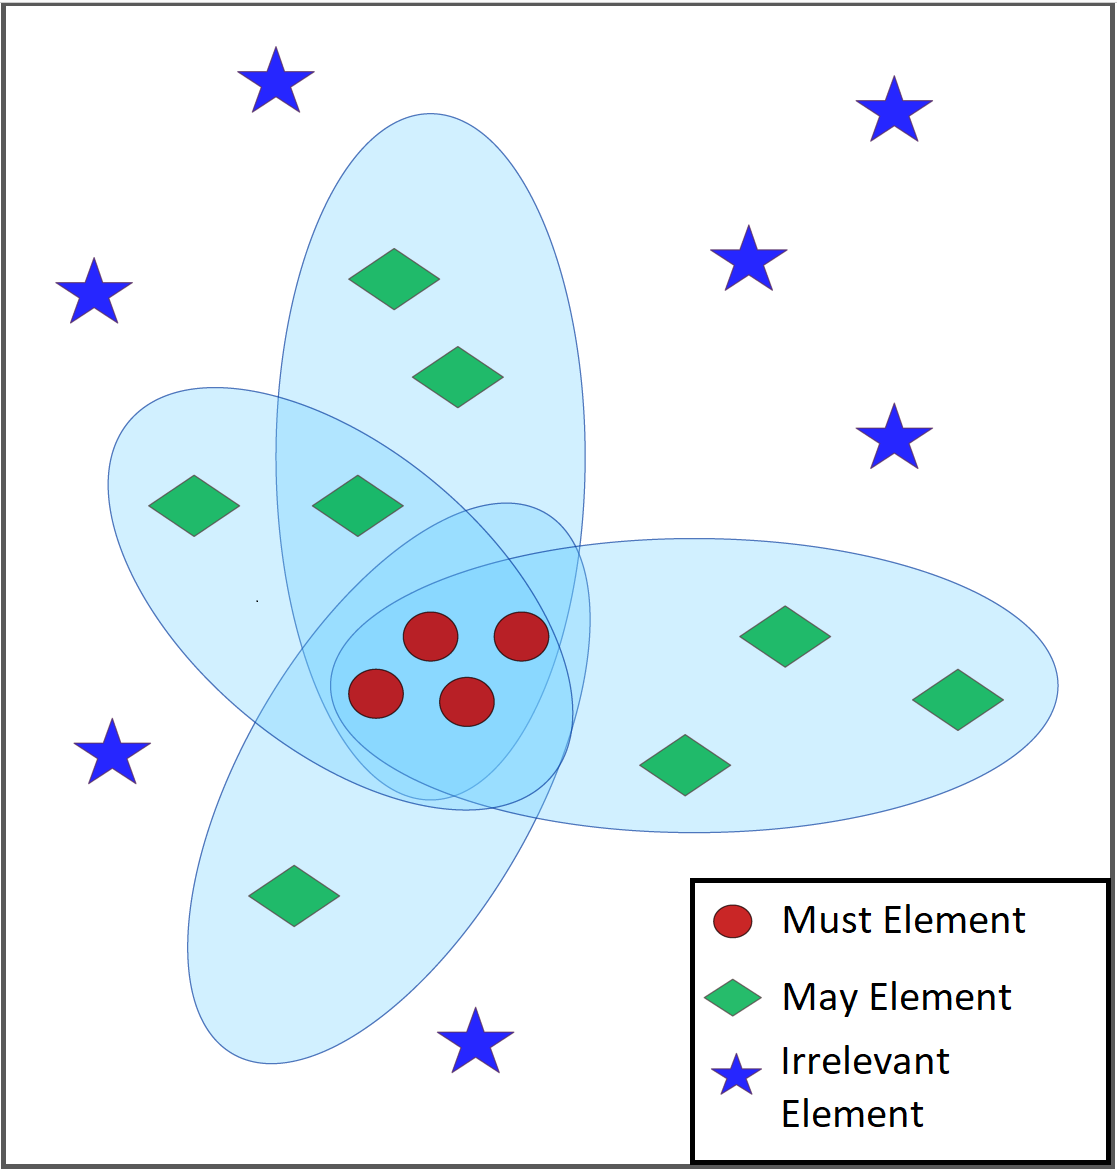
\includegraphics[scale=0.33]{figs/may_must_1.png}
\caption{Classification of Model Elements}\label{fig:maymust}
\end{center}
\end{figure}

Given all \mivc s, one gets a clear picture of the all possible ways that requirement is satisfied. This information helps categorize each target artifact into one of the following groups for that requirement.  The relationships are illustrated graphically in Figure~\ref{fig:maymust}, and explained formally below.
\begin{itemize}
  \item \textbf{MUST} elements - target artifacts that are present in all the \mivcs\ for a requirement (red circles in Figure~\ref{fig:maymust}).
      %$$ MUST_x = \{\forall i (S_xi \in \Sigma_x) \mid \bigcap S_xi \}$$
      $$ MUST (r) = \bigcap \ \aivc(r) $$

  \item \textbf{MAY} elements - target artifacts that are used in some, but not all, \mivcs\ (green diamonds in Figure~\ref{fig:maymust}).
      $$MAY(r) = (\bigcup \aivc(r)) \setminus MUST (r) $$

  \item \textbf{IRRELEVANT} elements - target artifacts that are not in any of the \mivcs\ (blue stars in Figure~\ref{fig:maymust}). $$IRR(r) = \Sigma \setminus (\bigcup \aivc(r))$$
\end{itemize}

This categorization helps identify the role and relevance of each target artifact in satisfying a requirement. The MUST elements are those target artifacts that are absolutely necessary for the requirement satisfaction. Hence, any change to these elements will most likely impact on each other. On the other hand, MAY elements indicate those target artifacts that satisfy the requirement in one of the possible ways.  Any change to just one of these elements will not affect the satisfaction of that requirement. The IRRELEVANT elements are never required to satisfy the requirement.

\subsubsection{Use of Traceability Information in Certification}
Safety-critical systems, like an airborne software, must undergo a rigorous software development process usually governed by particular standards, such as DO-178C for Software Considerations in Airborne Systems and Equipment Certification \cite{DO178C} and DO-333 for Formal Methods Supplement to DO-178C and DO-278A \cite{DO333}.
DO-178C proposes a rigorous software development process that starts with system-level requirements allocated to software, which are refined into high-level requirements, which are further refined into low-level requirements, source code, and finally, object code. For each kind of artifact, there are a set of {\em objectives} that should be met by critical avionics software.  The number of objectives and their rigor is determined by the {\em software level}, which is a measure of the criticality of the software and determined by a hazard assessment.

Three of the key tenets of this process are conformance, traceability and adequacy; that is, each refinement of an artifact must be traceable to the artifact if was derived from. Further, any additional functionality introduced within a layer that is not traceable to the layer above must be explained and justified.

DO-178C Section 5.5 describes {\em Software Development Process Traceability}, which requires that bi-directional traceability links exist between: system and high-level requirements (5.5a), high- and low-level requirements (5.5b), and low-level requirements and source code (5.5c).  The traceability links are designed for two purposes: to enable verification of the lower-level artifacts, and to give visibility into requirements added to lower levels of the hierarchy that are not directly traceable to requirements above them.
Section 6.3 describes Software Reviews and Analyses for each of the artifacts produced during software development.   The objective is to show that the higher-level artifacts are correctly developed into their lower-level equivalents.

%For example, Section 6.3.4.f states:
%\begin{quote}
%    Traceability: The objective is to ensure that the low-level requirements were developed into source code
%\end{quote}

Section 6.5 describes {\em Software Verification Process Traceability}, which provides bi-directional traceability between software requirements and tests.  Also, much of the focus of the Software Configuration Management Process activities in Chapter 7 are related to traceability; in particular Section 7.2.2 {\em Baselines and Traceability}, which describes traceability with respect to modifications of baselined software tools and libraries as well as {\em configuration items}, which are any items that are associated with the software development process for the software to be constructed.

The traceability ideas related to \mivcs\ can be applied to proofs between all levels and types of requirements and source code, but require that the requirements are formalized as called out in the DO-178C process.  There are 71 total objectives in DO-178C, of which 6 may be addressible by our technique, as shown in Table~\ref{tab:do178c}.  The traceability provided by \mivcs\ can demonstrate traceability between different layers of requirements and source code.  The determinant of success is the level of formality of the modeling effort for the system requirements and architecture.  If model checking is applied to show conformance of several architectural levels (as in~\cite{QFCS15:backes,hilt2013}), then traceability can be generated alongside the proof results.   In addition, the proof process itself can be used to address several more of the compliance objectives, but this is outside the scope of the current paper.

On the other hand, IVCs as currently conceived cannot be used to assist with traceability related to configuration management and software testing, as these aspects are not part of the proof process.  Interestingly, there are no specific traceability objectives in DO-178C associated with architecture and design activities, though there are other objectives related to conformance to requirements that are required.  In addition, at some level of abstraction, requirements become (of necessity) informal; at this level it is no longer possible to apply proof and so \mivcs\ cannot be derived.  We have not yet looked outside the DO-178 process to broader certification and safety concerns such as hazard analysis, but leave this as topic for future work.

\begin{table*}
  \caption{DO-178C Certification Objectives}
  \centering
  \begin{tabular}{ |c|c|c| }
    \hline
     Table Ref & Objective & Output  \\[0.5ex]
    \hline\hline
    Table A-2 (1) & High-level requirements are developed & Trace Data \\
    Table A-2 (4) & Low-level requirements are developed & Trace Data \\
    Table A-2 (6) & Source code is developed & Trace Data \\
    Table A-3 (6) & High-level requirements are traceable to system requirements & Software Verification Results \\
    Table A-4 (6) & Low-level requirements are traceable to high-level requirements & Software Verification Results \\
    Table A-5 (6) & Source code is traceable to low-level requirements & Software Verification Results \\
    \hline
  \end{tabular}
  \label{tab:do178c}
\end{table*}

\iffalse
DO-178C currently uses a variety of metrics to determine adequacy of requirements, but much of the effort involves code-level testing.  Test suites are derived from requirements and used to test the software and measured using different structural coverage test metrics.  If code-level test suites do not achieve full coverage, then an analysis is performed to determine whether there are missing requirements and test cases.  The kind of structural coverage required (e.g., statement, branch, MCDC) for adequate testing is driven by the criticality of the software in question.
\fi 

The utility of the IVCs are being evaluated by Rockwell Collins on a pilot project for both traceability and adequacy checking \cite{lucas17}. Previously, bi-directional traceability between artifacts involved tedious manual peer review to determine that requirements were adequate and that additional functionality was not introduced in the implementation model. IVCs offer automation to satisfy the DO-178C objectives related to traceability and adequacy, which is a very important use in providing certifications.


%, so neither does a change in these artifacts affect the satisfaction of the requirement, nor does a change in the requirement necessitate a change in these elements (at least in terms of satisfaction)



%Such proofs are not, in general, unique, and often there are multiple sets of clauses that could be used to construct a proof.  The existing traceability literature does not discuss multiple alternative satisfaction arguments or sets of trace links for one system design.

\iffalse
Instead of just recording the trace links from each requirement to the target artifacts, \emph{Satisfaction Arguments}~\cite{zave1997four,Hammond01:WiW} offer a semantically rich way to establish them.
A satisfaction argument attempts to establish that system requirements hold through an argument involving (i) the specification of the system behavior and (ii) assumptions about the domain of the system.
In ``Will it Work''~\cite{Hammond01:WiW}, Hammond et al. introduce rich traceability links to argue that subcomponent specifications together satisfy system requirements using structured (but informal) arguments.  These arguments are hierarchically organized, and component specifications at one level of hierarchy become requirement specifications for the component at the next lower level, as shown in Figure~\ref{fig:arch-fig}.

\begin{figure}
 \centering
  \includegraphics[ width=\columnwidth, trim = 70 170 75 0, clip=true ]{figs/arch-fig.pdf}
  \caption{Interplay between Architecture and Requirements}
  \label{fig:arch-fig}
  %\vspace{-0.1in}
\end{figure}


Proofs using model checking can be used to demonstrate satisfaction arguments.  Depending on the structure of the model and the properties to be proved, these proofs may demonstrate that an implementation conforms to a low-level specification~\cite{Miller10:CACM}, or that a lower-level specification conforms to a higher-level specification.  For the latter argument, assume-guarantee contracts~\cite{NFM2012:CoGaMiWhLaLu,Whalen13:WhatHow:TwinPeaksIEEESoftware} provide an appropriate mechanism for capturing the information needed from other modeling domains to reason about system-level properties.

In this formulation, guarantees correspond to the component requirements, and assumptions correspond to the environmental constraints that were used to verify that the component satisfies its requirements.  A contract specifies precisely the information that is needed to reason about the component’s interaction with other parts of the system. Furthermore, contract mechanism supports a hierarchical decomposition of verification process that follows the natural hierarchy in the system model.  For a given layer of the architecture, we use the contracts of the subcomponents within the architecture to establish the satisfaction of the system level requirements allocated to that level.  To create a complete proof, it is necessary to prove that each layer  establishes its system level property.

Although proofs can establish satisfaction arguments, from a traceability perspective, they are unsatisfactory.  With the baseline proof algorithms, it is not possible to establish which component-level requirements are necessary to establish a system property of interest.  However, \mivc s can be used to establish these kinds traceability relationships.  We have implemented this support into the AGREE
\fi


\iffalse


We call those target artifacts a \emph{set of support} for that requirement. Mathematically, if we think of the argument as a proof in which the requirement is the claim, then the set of support is the set of axioms (or clauses) that were necessary to prove the claim, and the trace links are means to associate the claim to those clauses. Such proofs are not, in general, unique, and often there are multiple sets of clauses that could be used to construct a proof.

There is substantial interest within the Requirements Engineering research community towards automating the construction and maintenance of traceability links~\cite{hayes2003improving, egyed2002automating,cleland2007best}.
%
%To that end, there are repositories such as the Data sets published at  Center of Excellence for Software Traceability~\cite{COEST} containing many example systems, each with a reasonably complete set of requirements and target artifacts and with trace links constructed by groups of experts.  It is then possible to benchmark automated and semi-automated traceability approaches against vetted sets of trace links.
%

We focus our attention to this subset of requirement traceability called {\em Satisfaction Arguments}~\cite{Hammond01:WiW} that are used to determine the portions of a design or model that are necessary to satisfy a functional requirement.
In fact, our work on IVCs was originally driven by the goal of automatically generating these trace links.

IVCs

automatically provide such arguments accurately and without human effort.

In addition, we can automatically generate expected artifact types, such as traceability matrices for these kind of relationships (see Figures~\ref{fig:propertyset1} and \ref{fig:propertyset4}).

%It is also the case, when computing all IVCs, that we can provide additional insight.  As far as we are aware, none of the existing Satisfaction Argument literature discusses the issue that there are often multiple satisfaction arguments between a requirement and its implementation.  Given all IVCs, it is possible to perform more accurate impact analysis and define multiple notions of requirements adequacy, as we will see in the following sections.

From a traceability perspective, these arguments help establish trace links (the \emph{satisfied by} relationship) between the requirements and those parts of the system and environment (the target artifacts) that were necessary to satisfy the requirements.

As originally conceived, these arguments describe functional relationships beween {\requirements}, {\em domain knowledge} , and {\em specifications}.


%Originally proposed by Zave and Jackson~\cite{zave1997four}, a satisfaction argument demonstrates how the behaviors of the system and its environment together satisfy the requirements.
%
%If the requirements and architecture efforts are based on natural-language requirements and modeling notations lacking rigorous semantics, the reasoning process we promote would closely resemble the Satisfaction Argument advocated by Hammond et al. in their outstanding paper “Will it work?” [12].

This has important ramifications for other forms of automatic trace link generation as pursued by the requirements engineering community.
For traceability research, the standard measures for examining the performance of different approaches is in terms of {\em precision} and {\em recall} against the ``gold standard'' set of traceability links that exist in predefined repositories.  Our concern is that, for requirements satisfaction traceability, there are often many such sets of valid links, as we have explored in this paper, so these metrics may be misleading.  One can envision situations in which the gold standard pursues one set of support and the automated approach pursues another, leading to low precision and recall scores.  A close examination of traceability links and categorizations such as the ones we have explored may be useful to provide more accurate measurements of the quality of automated approaches.
\fi
